% Tata letak bersama. Konten setiap bagian berada di sections/ dan appendices/.
\usepackage[T1]{fontenc}
\usepackage{lmodern}
\usepackage[bahasa]{babel}
\usepackage[margin=25mm,headheight=15pt]{geometry}
\usepackage{microtype}
\usepackage{graphicx,booktabs,tabularx,longtable,array}
\usepackage[table]{xcolor}
\usepackage{amsmath,enumitem,float,fancyhdr,titlesec,listings}
\usepackage{xurl}
\usepackage[section]{placeins}
\usepackage{needspace,etoolbox}
\pretocmd{\section}{\Needspace{6\baselineskip}}{}{}
\definecolor{Navy}{HTML}{17324D}
\definecolor{Teal}{HTML}{087F8C}
\definecolor{Pale}{HTML}{F0F5F8}
\definecolor{Muted}{HTML}{566573}
\usepackage[colorlinks=true,linkcolor=Navy,urlcolor=Teal,citecolor=Teal,bookmarksnumbered=true]{hyperref}
\hypersetup{pdftitle={IF4031 M1 - AkuAnakTehat},pdfauthor={Dzaky Aurelia Fawwaz; Muhammad Alfansya}}
\setlength{\parindent}{0pt}
\setlength{\parskip}{5pt}
\setlength{\emergencystretch}{3em}
\renewcommand{\arraystretch}{1.18}
\setlist{itemsep=2pt,topsep=4pt,leftmargin=*}
\newcolumntype{Y}{>{\raggedright\arraybackslash}X}
\newcolumntype{P}[1]{>{\raggedright\arraybackslash}p{#1}}
\titleformat{\section}{\Large\bfseries\color{Navy}}{\thesection}{0.7em}{}
\titleformat{\subsection}{\large\bfseries\color{Navy}}{\thesubsection}{0.7em}{}
\titleformat{\subsubsection}{\normalsize\bfseries\color{Teal}}{\thesubsubsection}{0.7em}{}
\pagestyle{fancy}
\fancyhf{}
\fancyhead[L]{\small IF4031\quad Milestone 1}
\fancyhead[R]{\small AkuAnakTehat}
\fancyfoot[L]{\scriptsize Platform Koordinasi Kebencanaan BNPB}
\fancyfoot[R]{\thepage}
\renewcommand{\headrulewidth}{0.3pt}
\raggedbottom
\lstdefinelanguage{Golang}{morekeywords={func,return,if,else,for,range,var,const,type,struct,map,select,case,default,go,defer,package,import,nil,true,false,continue},sensitive=true,morecomment=[l]{//},morestring=[b]"}
\lstset{basicstyle=\fontsize{8}{10}\selectfont\ttfamily,keywordstyle=\color{Navy}\bfseries,commentstyle=\color{Muted},stringstyle=\color{Teal},breaklines=true,breakatwhitespace=false,columns=fullflexible,keepspaces=true,showstringspaces=false,frame=single,rulecolor=\color{Navy!25},backgroundcolor=\color{Pale},numbers=left,numberstyle=\tiny\color{Muted},numbersep=6pt,xleftmargin=24pt,framexleftmargin=20pt,captionpos=b,tabsize=2}
\newcommand{\codepath}[1]{\href{\RepoURL/blob/\CodeRevision/#1}{\nolinkurl{#1}}}
\newcommand{\evidence}[1]{\codepath{docs/evidence/integration/#1}}
\newcommand{\reliabilityevidence}[1]{\href{\RepoURL/blob/\ReliabilityEvidenceRevision/docs/evidence/reliability-2026-10-08/#1}{\nolinkurl{docs/evidence/reliability-2026-10-08/#1}}}
\newcommand{\pending}[1]{\par\smallskip\noindent\fcolorbox{orange!60!black}{orange!7}{\parbox{0.93\linewidth}{\raggedright\textbf{Perlu dilengkapi.} #1}}\par\smallskip}
\newcommand{\diagram}[3]{\begin{figure}[htbp]\centering\includegraphics[width=\linewidth,height=0.76\textheight,keepaspectratio]{assets/figures/#1.pdf}\caption{#2}\label{#3}\end{figure}}
\newcommand{\architecturefigure}{\begin{figure}[H]\centering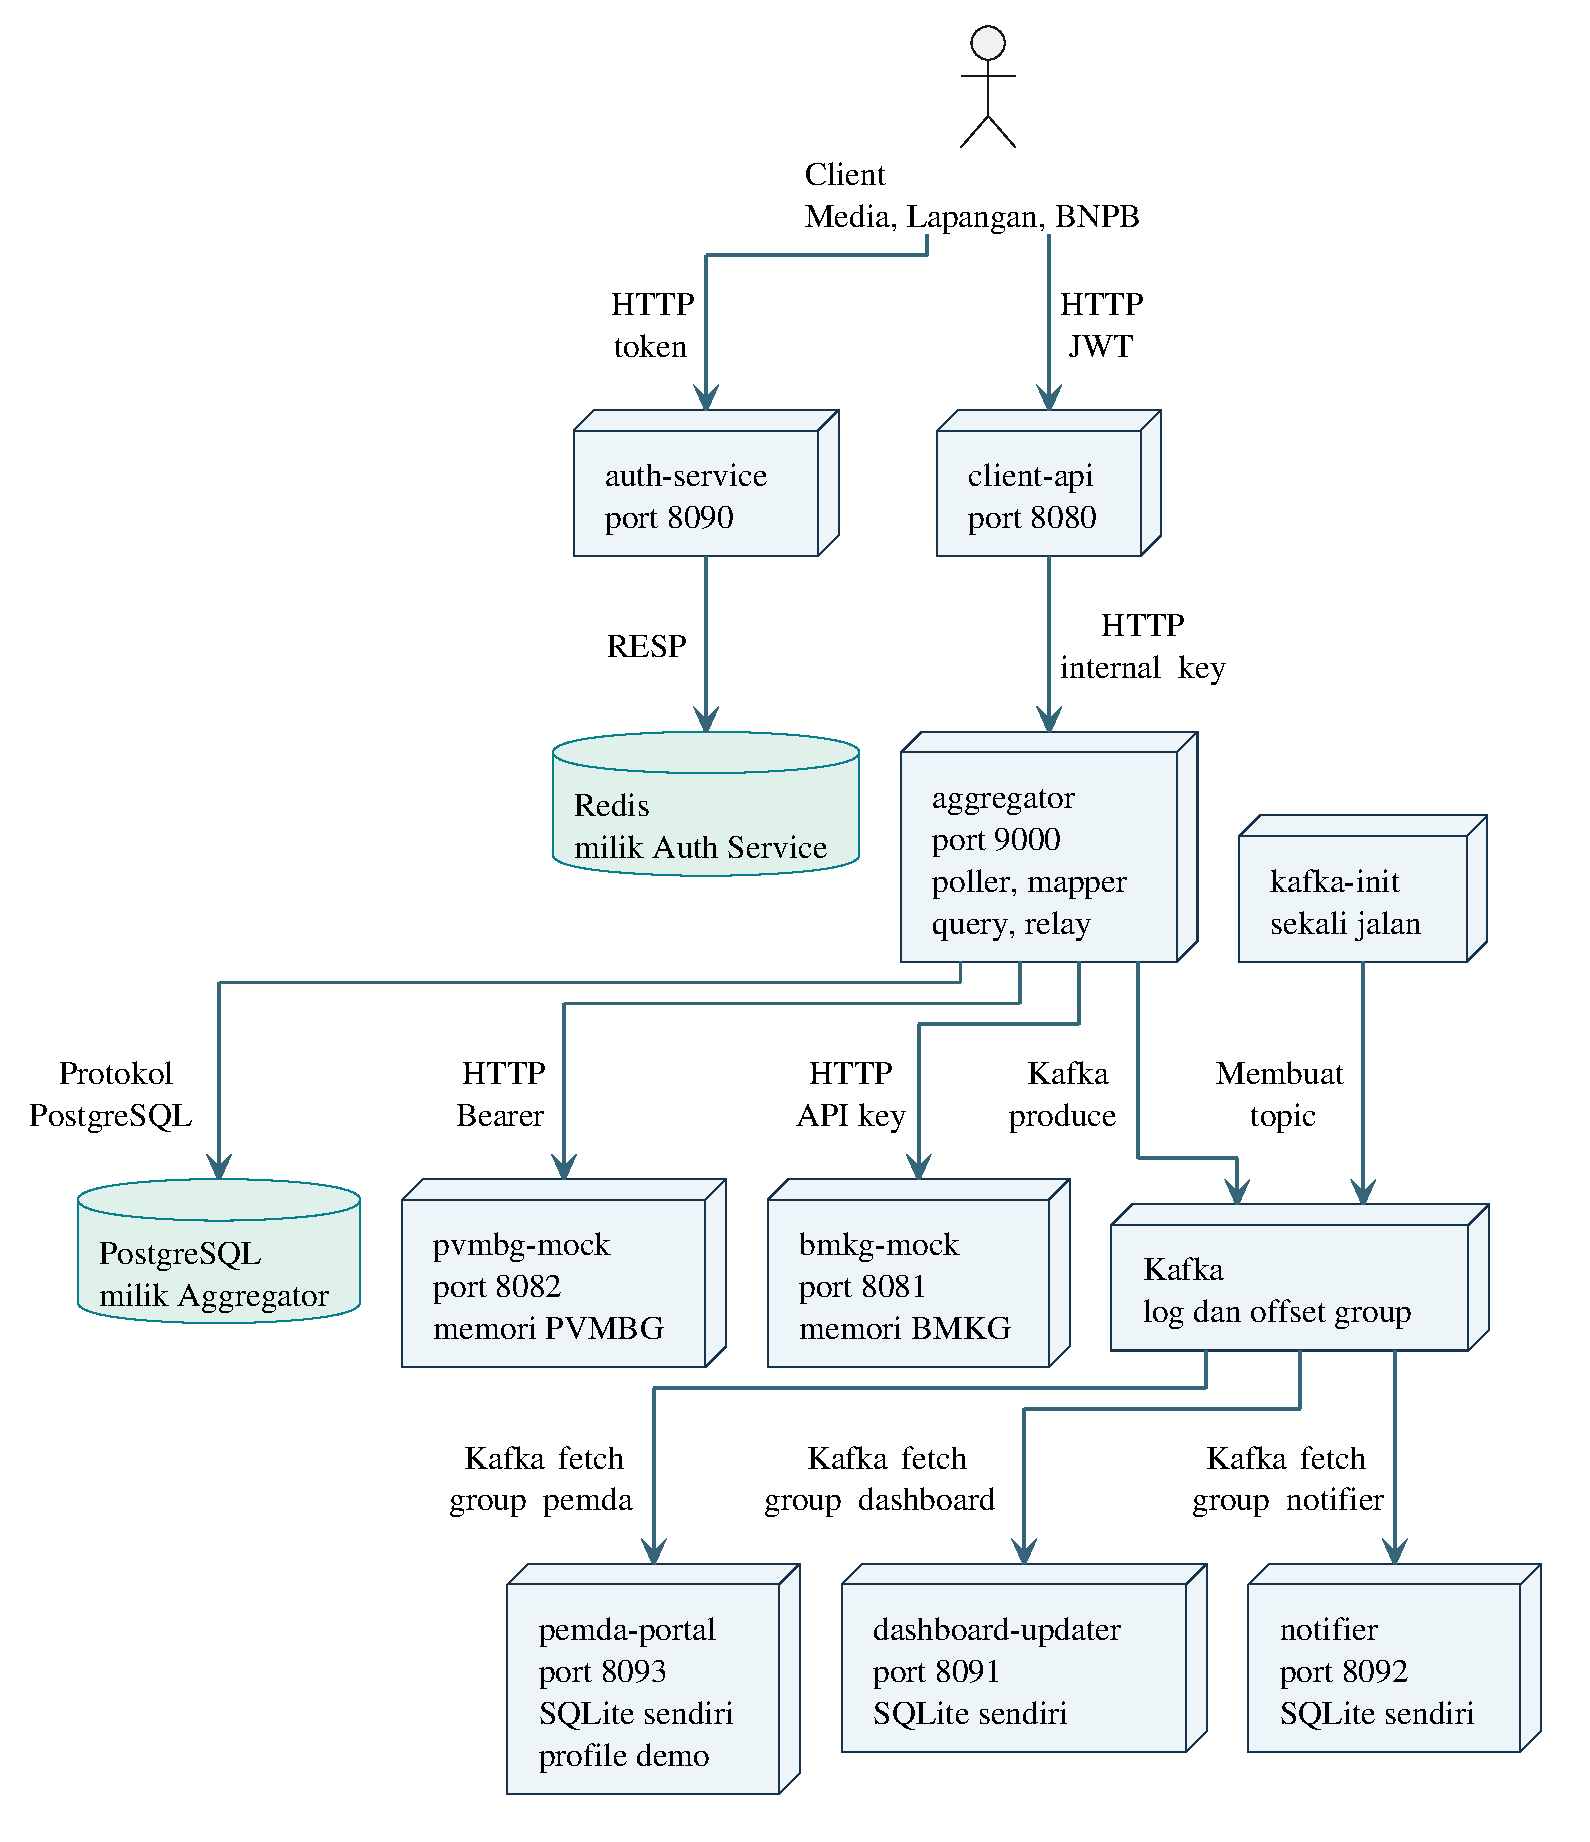
\includegraphics[width=\linewidth,height=0.74\textheight,keepaspectratio]{assets/figures/01-arsitektur.pdf}\caption{Arsitektur sistem beserta protokol dan kepemilikan penyimpanan. Setiap kotak dan simbol database mewakili satu container. Memori mock dan SQLite berada di dalam container pemilik. Panah dari Kafka menunjukkan aliran data menuju consumer yang menginisiasi fetch.}\label{fig:architecture}\end{figure}\clearpage}
\newcommand{\coderef}[1]{\par{\footnotesize Implementasi terkait terdapat pada \codepath{#1}.}\par}
\newcommand{\proof}[1]{\par{\footnotesize Bukti eksekusi tersedia pada \evidence{#1}.}\par}
\newcommand{\finalevidence}[1]{\href{\RepoURL/blob/\FinalEvidenceRevision/docs/evidence/final-2026-10-08/#1}{\nolinkurl{docs/evidence/final-2026-10-08/#1}}}
